\chapter{Hidden Markov Models}

\begin{itemize}
\item History, I guess...
\item Strengths and weaknesses on an intuitive level.
\item Strengths and weaknesses from the POV of morphologically rich
  languages.
\end{itemize}

\section{Example}
%\begin{itemize}
%\item Chained stochastic processes \citep{Rabiner1989}.
%\item The three classical problems of HMMs.
%\item Pioneered by \cite{Church1988} in POS tagging.
%\item The results by \cite{Brants2000} and \cite{Halacsy2007} probably
%  represent the generative state of the art.
%\item Very fast to train compared to discriminative models.
%\end{itemize}

I will illustrate Hidden Markov Models using an example. Imagine a
person called Jill who is hospitalized and occupies a windowless
room. The only way for her to know what is happening in the outside
world, is to observe a nurse who passes her room every day when she
comes to work\footnote{To make things simple, imagine the nurse never
  gets a day off.}.

Suppose, Jill is interested in weather phenomena and she decides to
pass time by guessing if it is raining outside. She bases her guesses
on whether or not the nurse is carrying an umbrella when she passes
the room. In other words, she predicts an unobserved variable, the
weather, based on an observed variable, the nurse's umbrella.

There are several probabilistic models Jill might use. The simplest
useful model assigns probability $1$ to the event of rain, if the
nurse carries an umbrella, and assign it the probability $0$
otherwise. This simplistic model would certainly give the correct
prediction most of the time, but Jill believes that she can do better.

Jill knows that people often carry an umbrella, when it is
raining. She also knows that they rarely carry one when the weather is
clear. However, people sometimes forget their umbrella at home,
perhaps because they are in a hurry. Moreover, people sometimes carry
an umbrella even when it is not raining. For example the weather might
be murky and they might anticipate rain. Therefore, Jill decides to
reserve some probability, say $0.2$, for the event that the nurse is
carrying an umbrella when the weather is clear. She reserves an equal
probability for the event that the nurse arrives at work without an
umbrella although it is in fact raining.
 
Without additional information, this more complicated model will give
exactly the same MAP predictions as the simplistic one. Knowledge of
meteorology, however, also factors in. Let us suppose Jill is a
weather enthusiast and she knows that the probability of rain is
$0.4$, making the probability of clear weather $0.6$. She also knows
that the probability of rain increases markedly on days following
rainy days at which time it is $0.7$.  Similarly, the probability of
clear weather increases to $0.9$ if the weather was clear on the
previous day. I summarize these probabilities in Table \ref{hmm-ex-1}.

\begin{table}[!htb]
\begin{center}
\begin{tabular}{|l|c|}
\hline
   i   &       \\
\hline
Clear  & $0.6$ \\
Rain   & $0.4$ \\
\hline
\end{tabular}~~~
\begin{tabular}{|l|cc|}
\hline
   T   & Clear & Rain  \\
\hline
Clear  & $0.9$ & $0.1$ \\
Rain   & $0.3$ & $0.7$ \\
\hline
\end{tabular}~~~
\begin{tabular}{|l|cc|}
\hline
   E    & No umbrella & Umbrella \\
\hline
Clear   & $0.8$ &  $0.2$         \\
Rain    & $0.2$ &  $0.8$         \\
\hline
\end{tabular}
\end{center}
\caption{Foo FIXME}\label{hmm-ex-1}
\end{table}

Let us assume that Jill observes the nurse for one week. She sees the
nurse carry an umbrella on all days except Tuesday. The MAP prediction
given by the simplistic model is that Tuesday is clear and all other
days are rainy. The more complex model will, however, give a different
MAP prediction: the probability is maximized by assuming that all days
are rainy. Under the more complex model, it is simply more likely that
the nurse forgot to take an umbrella on Tuesday.

\begin{figure}[!htb]
\begin{center}
\caption{Foo}\label{hmm-ex-2}
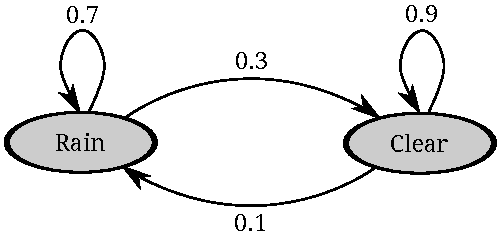
\includegraphics[scale=0.8]{hmm-ex-graph}
\end{center}
\end{figure}

The model Jill is using for weather prediction is called a Hidden
Markov Model. It can be used to make predictions about a series of
events based on indirect observations. 

The HMM is commonly visualized as a directed graph. Each hidden state,
for example Rain and Clear, represents a vertex in the
graph. Transitions from one hidden state to another are represented by
arrows labeled with probabilities. Figure \ref{hmm-ex-2} shows a graph
representing the transition structure of the HMM in Table
\ref{hmm-ex-1}.

\section{Formal Definition}

%\begin{itemize}
%\item Model derivation.
%\item Lexical model.
%\item First order transition model.
%\item Model order.
%\item Guesser for OOV words à la Brants.
%\end{itemize}

Abstracting from the example above, an HMM is a probabilistic model
that generates sequences of state-observation pairs. At each step $t$
in the generation process, the model generates an observation by
sampling the {\it emission distribution} of the current state
$y_t$. It will then generate a successor state $y_{t+1}$ by sampling
the {\it transition distribution} of $y_t$. The first hidden state $y_1$
is sampled from the {\it initial distribution} of the HMM.

Since we may assume that the succession of days is infinite, there was
no need to consider termination in the \ref{hmm-ex-2}. However, many
processes, such as sentences, do have finite duration. Therefore, a
special {\it final state} is required. When the process arrives at the
final state, it stops: no observations or successor states are generated.

Following \cite{Rabiner1989}, I formally define a {\it discrete} HMM
as a structure $(Y,\ X,\ i,\ T,\ E,\ F)$ where:
\begin{enumerate}
\item $Y$ is the set of hidden states ($Y = \{{\rm Clear},$ ${\rm Rain}\}$
  in the example in Table \ref{hmm-ex-1}).
\item $X$ is the set of emissions, also called observations ($\Sigma =
  \{{\rm Umbrella},$ ${\rm No\ umbrella}\}$ in the example in Table
  \ref{hmm-ex-1}).
\item $i: Y \rightarrow \R$ is the initial state distribution, that is the probability
  distribution determining the initial state of an HMM process (array
  i in Table \ref{hmm-ex-1}).
\item $T$ is the collection of transition distributions, $t_y: Y \rightarrow \R$, that
  determine the probability of transitioning from a state $y$ to each state
  $y'$ (array T in Table \ref{hmm-ex-1}).
\item $E$ is the collection of emission distributions $e_y: X
  \rightarrow \R$, which determine the probability of observing a
  particular emission $e \in X$ in hidden state $y \in Y$ (array $E$
  in Table \ref{hmm-ex-1}).
\item $f \in Y$ is the final state. The state $f$ emits no
  observations and there are no transitions from $f$.
\end{enumerate}
The definition of HMMs in this thesis work diverges slightly from
\cite{Rabiner1989} by introducing a final state. Final states were
used in for example \cite{foo}. Absorbing states \cite{bar} could also
be used. FIXME.

Figure \ref{hmm-ex-3} is a more accurate description of the HMM in
Table \ref{hmm-ex-1} than Figure \ref{hmm-ex-2}. The image has been
augmented with initial distribution and a final state. 

Because we assumed that the progression of days is infinite, the
probability of transitioning to the final state $f$ in example
\ref{hmm-ex-2} is 0 regardless of the current state. Hence, the
probability of any single sequence becomes 0. However, the probability
of an initial segment may still be non-zero\footnote{The probability
  of an initial segment up to position $t$ can be computed by
  marginalising over all infinite suffixes starting at $t$.}. For
example, the probability that the first three states are (Rain,
Rain, Clear) is X.

\begin{figure}[!htb]
\begin{center}
\caption{Foo}\label{hmm-ex-3}
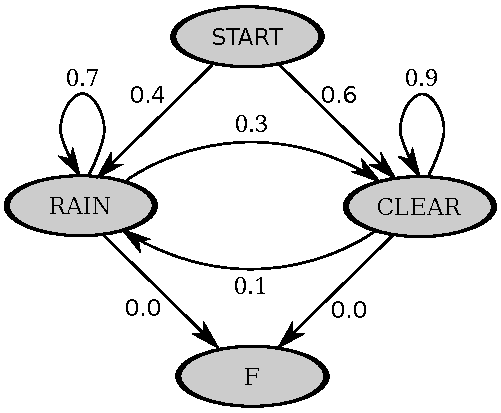
\includegraphics[scale=0.8]{hmm-ex-graph-2}
\end{center}
\end{figure}

I define a number of probabilities associated with an HMM:
\begin{enumerate}
\item The {\it joint probability} $p(x,y\parcond\theta)$ of a observation
  sequence $x$ and state sequence $y$. This is the probability that an
  HMM with parameters $\theta$ will generate the state sequence $y$
  and generate the observation $x_t$ in every state $y_t$.
\item The {\it total probability} $p(x\parcond \theta)$ of an observation
  sequence $x$. This is the probability that the observation sequence
  generated by the HMM is $x$.
\item The {\it conditional probability} $p(y\cond x\parcond\theta)$ of a
  state sequence $y$ given an observation sequence $x$. That is, how
  likely it is that the model passes through the states in $y$ when
  emitting the observations $x$.
\item The {\it marginal probability} $p(z, t\cond x\parcond \theta)$ of
  label $z$ at position $t$ given the observation sequence $x$. FIXME
\end{enumerate}

To formally define these probabilities, let $\theta = \{i,\ T,\ E\}$ be
the set of parameters of some HMM with observation set $X$ and hidden
state set $Y$, $x = (x_1,\ ...,\ x_T) \in X^T$ be a sequence of
observations and $y = (y_1,\ ...,\ y_T) \in Y^T$ a sequence of hidden
states (having the same length as $x$). Then the joint probability
$p(x,y;\theta)$ of $x$ and $y$ given $\theta$ is defined by Equation
\eqref{hmm-joint-prob}.
\begin{equation}
p(x,y\parcond\theta) = i(y_1) \cdot \Bigg( \prod_{t = 1}^{T-1} t_{y_t}(y_{t + 1})\Bigg) \cdot t_{y_T}(f) \cdot \prod_{t = 1}^T e_{y_t}(x_t)\label{hmm-joint-prob}
\end{equation}
Equation \eqref{hmm-joint-prob} is a product of two factors: the
probability of the hidden state sequence $y$, determined by the
initial and transition probabilities, and the probability of the
emissions $x_t$ given hidden states $y_t$ determined by the emission
probabilities.

There is no limit on the number of hidden states in $Y$ that can emit
an observation $x_t$. Therefore, it is quite possible that the same
observation sequence $x$ can be generated from many different state
sequences. The total probability $p(x\parcond\theta)$ of an observation
sequence $x$ can be found by summing over all state sequences that
could have generated $x$. It is defined by Equation
\eqref{hmm-obs-prob}.
\begin{equation}
p(x\parcond\theta) = \sum_{(y_1,\ ...,\ y_T) \in Y^T} p(x, y\parcond \theta)\label{hmm-obs-prob}
\end{equation}

Possibly the most important probability associated to the HMM is the
conditional probability $p(y\cond x\parcond\theta)$ of state sequence $y$
given observations $x$. This is an important quantity because
maximizing $p(y\cond x\parcond\theta)$ with regard to $y$ will give the MAP
assignment of observation sequence $x$. It is defined by Equation
\eqref{hmm-cond-prob}.
\begin{equation}
p(y\cond x\parcond\theta) = \frac{p(x,y\parcond\theta)}{p(x\parcond\theta)}\label{hmm-cond-prob}
\end{equation}

Finally, the posterior marginal probability of state $z$ at position $t$ given
the observation sequence $x$ is computed by summing, or marginalizing,
over all state sequence $y$, where $y_t = z$. It is defined by
Equation \eqref{hmm-marg-prob}
\begin{equation}
p(z, t\cond x\parcond \theta) = \frac{\sum_{(y'_1,\ ...,\ y'_T) \in Y^T, y'_t = z} p(x, y'\parcond \theta)}{p(x\parcond\theta)}\label{hmm-marg-prob}
\end{equation}

\section{Inference}
%\begin{itemize}
%\item The forward algorithm.
%\item Guarding against underflow: Dynamic scaling \citep{Rabiner1989} or exp-sum-log \citep{Durbin1998}.
%\item The Viterbi algorithm.
%\item Fixed beam search.
%\item Determining the beam: fixed, threshold and adaptive beam \citep{pal2006}.
%\item The forward-backward algorithm and multitagging.
%\end{itemize}
Informally, inference in HMMs means finding a maximally
probable sequence of hidden states $y$ that might have emitted the
observation $x$. As \cite{Rabiner1989} points out, this statement is
not strong enough to suggest an algorithm. 

Maximally probable is an ambiguous term when dealing with structured
models. It could be taken to mean at least two distinct things. The
MAP assignment $y_{MAP}$ of the hidden label sequence is the most
probable joint assignment of labels defined by Equation
\eqref{hmm-map}. Another possible definition would be the {\it maximum
  marginal} (MM) assignment. It chooses the most probable hidden
state for each word regardless of the states of all other words. The
MM assignment $y_{MM}$ is defined by Equation \eqref{hmm-mm}.

\begin{equation}
y_{MAP} = \argmax_{y\in Y^T} p(y\cond x\parcond\theta)\label{hmm-map}
\end{equation}

\begin{equation}
y_{MM} = \argmax_{y\in Y^T} \prod_{t = 1}^T p(y_t, t \cond x\parcond\theta)\label{hmm-mm}
\end{equation}

As \cite{Merialdo1994} and many others have noted, the MAP and MM
assignments maximize different objectives. The MM assignment maximizes
the accuracy of correct states per observations whereas the MAP
assignment maximizes the number of completely correct state
sequences. Both objectives are important from the point of view of POS
tagging. However, they are often quite correlated and, at least in POS
tagging, it does not matter in practice which of the criteria is used
\citep{Merialdo1994}. Most systems, for example
\cite{Church1988,Brants2000,Halacsy2007}, have chosen to use MAP
inference.

Although, MM inference is more rarely used with HMMs, computing the
marginals is important both in unsupervised estimation of HMMs and
discriminative estimation of sequence models. Therefore, I will
present this algorithm as well.

There are a number of strongly related algorithms for both exact MAP
and MM inference. I use the Viterbi algorithm for MAP inference and
the forward-backward algorithm for MM inference
\citep{Rabiner1989}. Belief propagation introduced by \cite{Peral1982}
computes the MM assignment and can be modified to compute the MAP
assignment as well. For sequence models, belief propagation is very
similar to the forward-backward algorithm. It can, however, be
extended to cyclic graphs \citep{Weiss2000}. 

Since cyclic models fall beyond the scope of this thesis and both the
Viterbi and forward-backward algorithms are amenable to well known
optimizations, which are of great practical importance, I have chosen
to omit belief propagation. I refer to \cite{Koller2009} for a nice
treatment of belief propagation and graphical models at large.

Before introducing the Viterbi and forward-backward algorithm, I am
going to explain the forward algorithm, which is used to compute the
total probability of an observation and also as part of the
forward-backward algorithm.

\begin{figure}[!p]
\begin{center}
\caption{foo.}\label{hmm-trellis}
\begin{subfigure}{\textwidth}
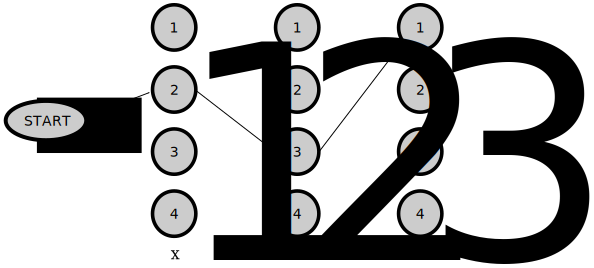
\includegraphics[scale=0.65]{trellis_path}
\caption{Trellis and path.}\label{hmm-ex-trellis-path}
\end{subfigure}
\vskip.5cm
\begin{subfigure}{\textwidth}
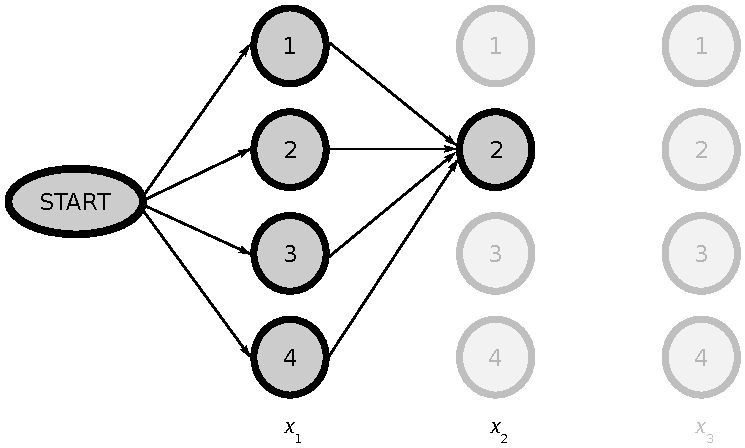
\includegraphics[scale=0.65]{trellis_forward}
\caption{Forward path prefixes.}\label{hmm-ex-trellis-fw}
\end{subfigure}
\vskip.5cm
\begin{subfigure}{\textwidth}
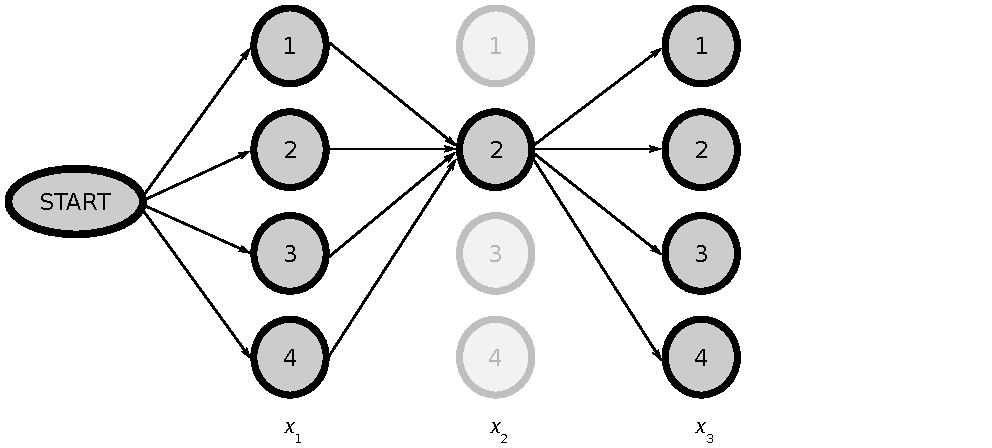
\includegraphics[scale=0.65]{trellis_marginal}
\caption{Marginal paths.}\label{hmm-ex-trellis-marginal}
\end{subfigure}
\end{center}
\end{figure}

\subsection{The Forward Algorithm}

Equations \eqref{hmm-map} and \eqref{hmm-mm} reveal, that both MAP
and MM inference require knowledge of the entire observation $x$. In
the weather prediction example, the observation is, however, always
infinite. What kind of inference is possible in this case?

Even when we only know a prefix $x[1:t]$ (of length $t$) of the entire
observation $x$, we can still compute the {\it belief state}
\citep{foo} of the HMM given the prefix. The belief state is in fact
not a single state, but rather a distribution over the set of hidden
states $Y$. It tells us how likely we are to be in a given state
$z$ when we have emitted the prefix $x[1:t]$.

To compute the belief state at position $t$, we first need to compute
the {\it forward probabilities} for each state $z \in Y$. The forward
probability $f_{t,z}(x)$ of state $z$ at position $t$ is the
probability of emitting prefix $x[1:t]$ and ending up in state $z \in
Y$. For example, given the infinite observation $x = (${\sc umbrella},
{\sc umbrella}, {\sc no umbrella},\ ...$)$, the forward probability
$f_{3,\textsc{rain}}$ is the probability that the third day is rainy,
when the nurse had an umbrella on days one and two, but did not have
one on the third day.

Conceptually, the forward probability is computed by summing over all
path prefixes up to position $t$, where the state at position $t$ is
$z$, see Figure \ref{hmm-ex-trellis-fw}. Formally, the forward
probability is defined by Equation \eqref{forward_prob}.
\begin{equation}
f_{t,z} = \sum_{y\in Y^t} \Bigg(i(y_1) \cdot \Bigg(\prod_{u = 1}^{t - 1} t_{y_u}(y_{u + 1}) \Bigg) \cdot \prod_{u = 1}^t e_{y_u}(x_u)\Bigg)\label{forward_prob}
\end{equation}
Comparing Equations \eqref{forward_prob} and \eqref{hmm-joint-prob}
shows that the forward probability represents a prefix of the
probability path probability $p(x, y \parcond \theta)$.

The belief state and posterior marginal distribution may seem
similar. They are, however, distinct distributions because the belief
state disregards all information about observation $x$ after position
$t$. In contrast, the marginal distribution encompasses information about
the entire observation. For example the marginal probability of {\sc
  rain} at position 3 is likely to depend strongly on whether we
observe {\sc umbrella} on day 4, or not. However, this will have no
impact on the belief state.

Figure \ref{fw-naive-prob} demonstrates a naive approach to computing
the forward probabilities. Simply list all relevant state sequences,
compute the probabilities of each sequence and sum
them. Unfortunately, the naive approach fails for large $t$ because
the number of distinct state sequences depends on the sequence length
in an exponential manner.

The complexity of the naive algorithm is $|Y|^t$, which is infeasible.
For example, $f_{20,\textsc{rain}}(x)$ requires us to sum
approximately 20 million probabilities and $f_{30,\textsc{rain}}(x)$
entails summation of approximately 540 million probabilities. Since
observations in domains such as natural language processing frequently
reach lengths of $100$, a more efficient approach is necessary.

\begin{figure}[!ftb]
\begin{center}
\caption{foo}\label{fw-naive-prob}
\begin{tabular}{lllr}
$y_1$ & $y_2$ & $y_3$ & $p$ \\
\hline
{\sc clear} & {\sc clear} & {\sc clear} & $(0.6\cdot0.8\cdot0.9\cdot0.2)\cdot0.9\cdot0.8\approx0.062$\\
{\sc rain}  & {\sc clear} & {\sc clear} & $(0.4\cdot0.2\cdot0.3\cdot0.2)\cdot0.9\cdot0.8\approx0.003$\\
{\sc clear} & {\sc rain}  & {\sc clear} & $(0.6\cdot0.8\cdot0.1\cdot0.8)\cdot0.3\cdot0.8\approx0.009$\\
{\sc rain}  & {\sc rain}  & {\sc clear} & $(0.4\cdot0.2\cdot0.7\cdot0.8)\cdot0.3\cdot0.8\approx0.011$\\
& & & \\
%\hline
%\vspace{0.1cm}
~~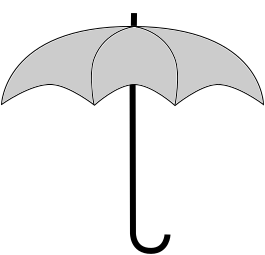
\includegraphics[width=0.5cm]{umbrella} & ~~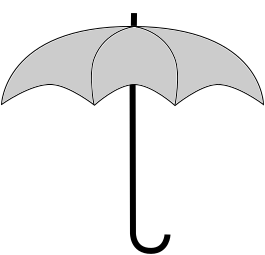
\includegraphics[width=0.5cm]{umbrella} & ~~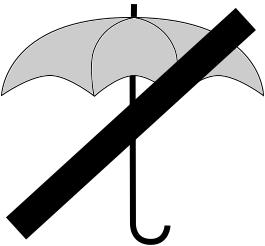
\includegraphics[width=0.5cm]{no_umbrella} & \\
\hline
        &       & & $\approx0.086$
\end{tabular}
\end{center}
\end{figure}

The belief state can be computed in linear time with regard to $t$
using the {\it forward algorithm} \citep{Rabiner1989}, which is in
fact simply a recursive application of the right distributive rule of
algebra
$$a_1 \cdot b + ... + a_n \cdot b = (a_1 + ... + a_n)\cdot b$$
for real numbers $a_1$ up to $a_n$ and $b$. 

Instead of computing the probability separately for each path, the
forward probabilities for longer paths are computed incrementally
using the forward probabilities of shorter paths. Examine Figure
\ref{fw-naive-prob}. By grouping rows one and two, as well as three
and four into pairs, it is easy to see that
$$f_{3,\textsc{clear}} = (f_{2, \textsc{rain}}\cdot t_{\textsc{rain}}(\textsc{clear}) + f_{2, \textsc{clear}} \cdot t_{\textsc{clear}}(\textsc{clear})) \cdot e_{\textsc{clear}}(\textsc{no\ umbrella})$$
Generalizing, we get the recursion in Equation \eqref{fw-rec}.
\begin{equation}
f_{t, z} = \left\{
\begin{aligned}
&i(z) \cdot e_{z}(x_1)  & , &\  t = 1\\
&\Bigg(\sum_{z'\in Y} f_{t - 1, z'}\cdot t_{z'}(z) \Bigg) \cdot e_{z}(x_{t}) & ,&\ 1 < t \le T\\
&\sum_{z'\in Y} f_{T, z'}\cdot t_{z'}(F) & ,&\  t = T + 1,\ z = F.
\end{aligned}
\right.
\label{fw-rec}\end{equation}

The base case in Equation \eqref{fw-rec}, for $t = 1$, has no
transition probability, but it does have the initial probability. The
forward probability $f_{T + 1, F} = p(x \parcond \theta)$. In fact one
of the principal applications for the forward algorithm is computing
the total probability of an observation. The other application is as
part in computing the marginal distributions over positions.
  
The forward algorithm is outlined in Algorithm
\ref{forward-algorithm}. Assuming that accessing the data structures
{\tt x}, {\tt i_prob}, {\tt e_prob}, {\tt tr_prob} and {\tt trellis}
is constant time, the complexity of the algorithm is dominated by the
three nested loops on lines \ref{start-cplx} up to
\ref{stop-cplx}. This shows that the complexity of the forward
algorithm is linear with regard to the length of the sequence and
quadratic with regard to the hidden state set.

\begin{algorithm}[!p]
\caption{The forward algorithm in Python 3.}\label{forward-algorithm}
\begin{lstlisting}
def forward(x, i_prob, e_prob, tr_prob): 
    """
        x       - The observation as a list.
        i_prob  - Initial state distribution.
        e_prob  - Emission distributions.
        tr_prob - Transition distributions.

        Return the trellis of forward probabilities. 
    """

    assert(not x.empty()) 

    trellis = {}

    # Indexing in python starts at 0.
    x_1 = x[0]
    T   = len(x) + 1

    # Set final state F. States are consequtive integers 
    # in the range [0, F]. 
    F = len(i_prob) - 1 

    # Initialize first trellis column.
    for z in range(F):
        trellis[(1,z)] = i_prob[z] * e_prob[z][x_1]

    # Set all except the final column.(*@\label{start-cplx}@*)
    for t in range(2, T):
        trellis[(t, z)] = 0

        x_t = x[t - 1]

        for z in range(F):
            for s in range(F):
                trellis[(t, z)] = (trellis[(t - 1, s)] * 
                                   tr_prob[s][z])

            trellis[(t, z)] *= em_prob[z][x_t](*@\label{stop-cplx}@*)

    # Set the last column.
    for z in range(s_count):
        trellis[(T + 1, z)] = trellis[(T, z)] * tr_prob[z][F]

    return trellis
\end{lstlisting}
\end{algorithm}


\subsection{The Viterbi Algorithm}
\label{hmm-viterbi}

\subsection{The Forward-Backward Algorithm}
\label{hmm-fw-bw}

\section{Estimation}
%\begin{itemize}
%\item Counting vs Baum-Welch.
%\item Smoothing over orders.
%\item Smoothing missing counts.
%\item Estimating parameters for OOV word model.
%\end{itemize}

HMMs can be trained in different ways depending on the quality of the
available data, but also on the task at hand. The classical setting
presented by \cite{Rabiner1989} is nearly completely unsupervised: the
HMM is trained exclusively from observations. Some supervision is
nevertheless usually required to determine the number of hidden
states\footnote{Although methods for determining the number of states
  from the data exist \citep{foo}.}. Additionally priors on the
emission and transitions distributions may be required to avoid
undesirably even distributions
\citep{Cutting1992,Johnson2007}.

The unsupervised training setting has two important and
interrelated applications:
\begin{enumerate}
\item Modeling a complex stochastic process from limited data. Here
  the HMM can be contrasted to a Markov chain \citep[318--320]{Manning1999}, where
  each emission can occur in a unique state leading to a higher degree
  of data sparsity and inability to model under-lying structure.
\item Uncovering structure in data, for example part-of-speech
  induction \citep{Johnson2007}.
\end{enumerate}
The classical method for unsupervised Maximum likelihood estimation of
HMMs is the {\it Baum-Welch algorithm} \citep{Rabiner1989}, which is
an instance of the {\it expectation maximization algorithm} (EM)
\citep{Dempster1977} for HMMs.

\section{HMM taggers and Morphological Analyzers}
\begin{itemize}
\item Limiting transitions.
\item How much of an improvement can be expected?
\end{itemize}


\section{HMMs for POS Tagging}

\section{Problems}
\begin{itemize}
\item Local normalization.
\item Inability to use word context.
\item Label bias.
\item The inability to use rich features, causes problems in domains
  other than POS tagging and in POS tagging for MR languages.
\item Smoothing is difficult.
\item Differences in performance between generative HMMs and
  discriminative approaches are even greater for morphologically
  complex languages and small training sets.
\item OOV words may require different mechanisms depending on
  language again causing problems for MR lanuages.
\end{itemize}

\section{Enriching the emission and transition models}
\begin{itemize}
\item \cite{Halacsy2007} and \cite{Silfverberg2011}.
\end{itemize}
